
\chapter{Software Design, Implementation, and Validation}
\label{chap:implementation}

\section{Analysis and Design Goals}

Because the thesis contains an implemented software system, the written document should reflect the essential stages of the application life cycle: analysis, design, implementation, and testing. In this project, the analysis stage identified four non-negotiable requirements. First, the system had to preserve strict alignment between each fMRI sample and its visual target. Second, it had to support rapid experimental iteration without silently changing the evaluation protocol. Third, it had to make it easy to compare model versions under a common metric suite. Fourth, it had to remain reproducible enough that every reported result could be traced back to a concrete configuration and checkpoint.

These requirements informed the high-level design of the pipeline. Instead of building a monolithic training script, the system was organized around loosely coupled stages: data preparation, target extraction and caching, model training, evaluation, result aggregation, and qualitative analysis. This decomposition reduces implementation risk and makes scientific debugging more transparent. If an experiment fails, the author can determine whether the failure is caused by preprocessing, target generation, optimization, or evaluation rather than treating the whole project as a black box.

\section{Software Architecture}

At a conceptual level, the implemented system follows a staged architecture:
\begin{enumerate}[leftmargin=1.8em]
    \item \textbf{Data layer:} loading NSD-derived features, image identifiers, subject/session metadata, and split definitions;
    \item \textbf{Target layer:} extracting, caching, and reusing CLIP-based latent targets and derived variants;
    \item \textbf{Model layer:} defining baseline and multi-head decoders together with their losses and optimization logic;
    \item \textbf{Evaluation layer:} computing retrieval metrics, shortlist reranking, fusion scores, and summary tables;
    \item \textbf{Analysis layer:} storing experiment manifests, qualitative outputs, plots, and leaderboard-style comparisons.
\end{enumerate}

This architecture is intentionally research-oriented. Its purpose is not only to train a model, but also to preserve experimental meaning and make repeated ablations comparable.

\begin{figure}[htbp]
    \centering
    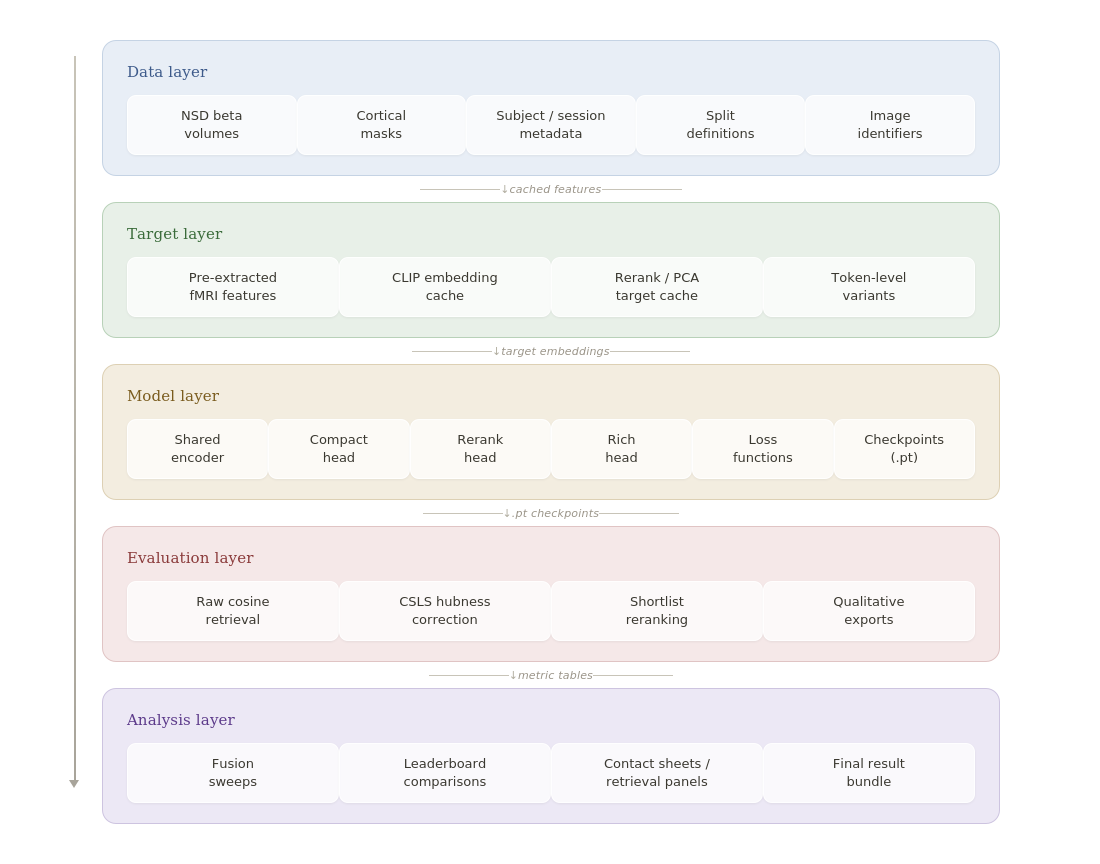
\includegraphics[width=0.92\textwidth]{software_architecture.png}
    \caption{Software architecture of the research pipeline. The implementation is deliberately layered so that data preparation, target caching, training, evaluation, and qualitative export remain traceable and reproducible.}
    \label{fig:software_architecture}
\end{figure}

\section{Configuration Management and Versioning}

A recurring difficulty in research software is that experiments drift over time: hyperparameters change, split definitions evolve, and intermediate artifacts are overwritten. To avoid this, the pipeline is organized around versioned experiment configurations. Each major experiment wave is associated with an explicit configuration file that records data sources, target choices, architecture hyperparameters, loss weights, training settings, and evaluation options.

Versioning is especially important in this thesis because the experimental narrative depends on comparing multiple iterations rather than reporting only a single final run. When a new idea is tested, the goal is not merely to obtain a number but to understand whether a change in the score is caused by the underlying modelling idea or by a hidden change in the protocol. Configuration versioning therefore supports both reproducibility and interpretability.

\section{Implementation of the Training and Evaluation Flow}

The implementation flow can be summarized as follows. First, NSD-derived samples are loaded and normalized under a split-aware preprocessing regime. Second, target latents are either extracted on demand or retrieved from caches, reducing repeated compute and eliminating inconsistencies between experiments. Third, the selected decoder is trained with a loss appropriate to the experiment family. Fourth, validation-time retrieval is computed on a fixed gallery, together with CSLS correction and shortlist reranking when applicable. Finally, results are aggregated into human-readable summaries and compared against previous runs.

A useful abstraction is to think of the whole system as a deterministic map
\begin{equation}
\mathcal{P}:(\mathcal{D},\mathcal{C},\mathcal{A}) \longmapsto \mathcal{R},
\label{eq:pipeline_map}
\end{equation}
where $\mathcal{D}$ denotes the data and split definition, $\mathcal{C}$ the configuration, $\mathcal{A}$ the cached artifacts and checkpoints, and $\mathcal{R}$ the resulting metrics and qualitative outputs. The advantage of this view is that it clarifies what must remain fixed when two experiments are compared.

\section{Validation and Testing Strategy}

In the present project, testing took several complementary forms:
\begin{itemize}
    \item \textbf{split-integrity checks}, ensuring that repeated images or derived artifacts cannot leak across train and validation sets;
    \item \textbf{shape and alignment checks}, verifying that every prediction matrix corresponds exactly to its intended ground-truth target matrix;
    \item \textbf{metric sanity checks}, confirming that retrieval metrics behave as expected on controlled inputs;
    \item \textbf{checkpoint and cache verification}, ensuring that the correct artifacts are loaded during evaluation;
    \item \textbf{qualitative inspection}, used to detect failure modes that aggregate metrics can hide.
\end{itemize}

This testing strategy is substantial enough to be regarded as part of the thesis contribution. Several improvements in the final system did not come from inventing a new loss function, but from identifying and eliminating hidden sources of inconsistency. In that sense, rigorous validation acted as a performance multiplier.

\begin{figure}[htbp]
    \centering
    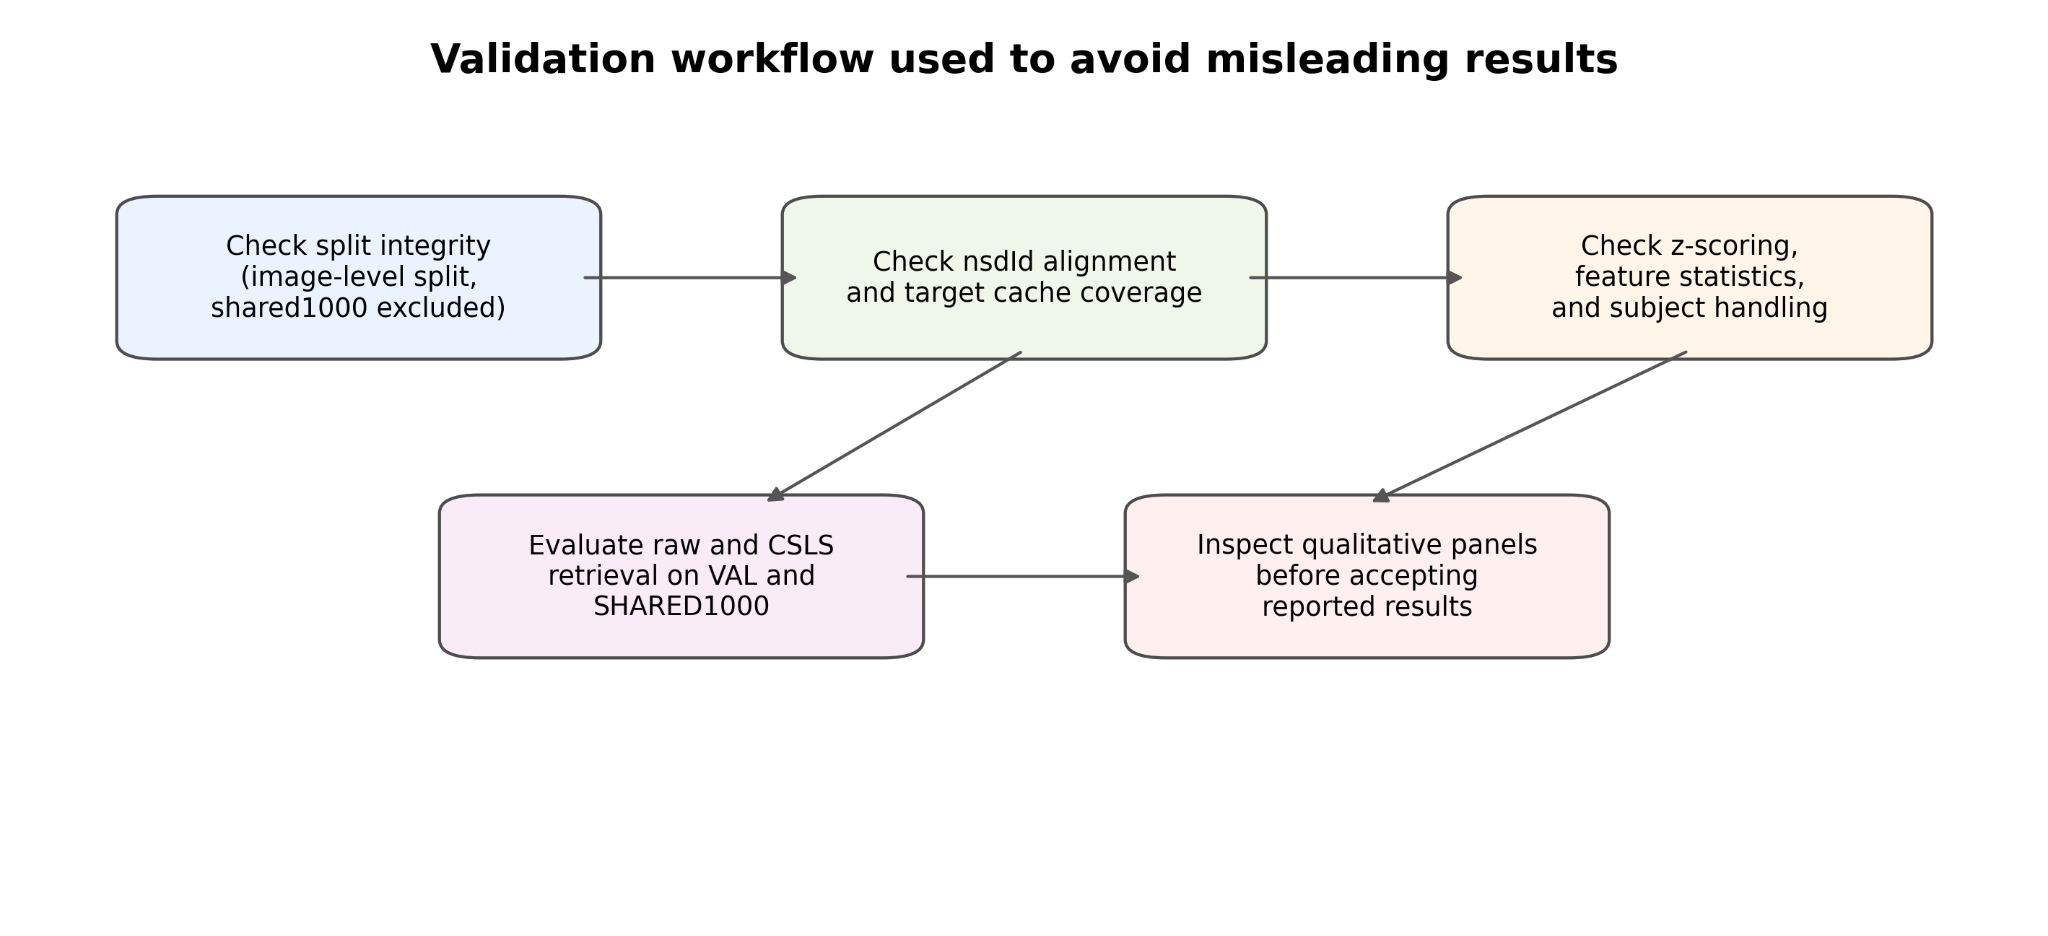
\includegraphics[width=0.95\textwidth]{validation_workflow.png}
    \caption{Validation workflow used throughout the thesis. Raw metric values are only trusted after split integrity, alignment, normalization, and qualitative inspection have been verified.}
    \label{fig:validation_workflow}
\end{figure}

\section{Reproducibility, Artifact Management, and Reporting}

Reproducibility in this thesis is supported by explicit artifact management. Targets, checkpoints, predictions, and summary outputs are stored as named and versioned artifacts. This makes it possible to revisit a result months later and still recover its provenance. Such traceability is essential in a long-running experimental project, especially when results evolve across many versions.

The reporting layer is equally important. Tables, plots, retrieval examples, and diagnostic summaries are not treated as cosmetic additions but as part of the scientific record. For example, a metric table may reveal that rerank-only retrieval underperforms globally, while a shortlist-local diagnostic may show that the rerank head still contains useful discriminative information. Only by keeping both artifact provenance and reporting structure under control can such nuanced conclusions be justified.

